\section{A motivating example: parkinson's disease}
\label{intro-complete_ex}

need for confrontation
heterogeneous data

spline
heterogeneous data and overlapping age groups \ref{applications-age_groups} \ref{theory-age_group_model-overlapping_data}
study level fixed effects (diagnostic criteria) \ref{applications-efx_study_level} \ref{theory-covariate_modeling}
country level fixed effects (representative) \ref{applications-efx_country_level} \ref{theory-covariate_modeling}
random effects \ref{applications-rfx} \ref{theory-covariate_modeling}
csmr v pf \ref{applicatoins-csmr} \ref{theory-csmr}

x_cv_ascertainment
x_cv_diagnostic_criteria
x_cv_representative
x_ihme_fao_stimulants_kcal_26oct11
x_smoking_prev

complete discussion of all p, i and pf data points

chronic neurodegenerative disorder
are effective symptomatic therapies
no treatment has yet been identified that would significantly slow its natural progression
motor dysfunction in early stages
non-motor symptoms: dementia, sleep-wake cycle dysregulation and autonomic failure

Symptomatic therapy with dopamine replacement strategies is associated with marked improvement of motor symptoms and disability but has not been shown to significantly alter
the progression of the underlying neuronal degeneration of illness

After prolonged disease duration of 10 or more years a majority of patients will
also have developed a plethora of non-motor symptoms for which there are currently no effective treatments. These include cognitive decline, dementia and psychosis, autonomic failure, sleep-wake-cycle dysregulation as well as depression, pain and sensory symptoms

progression of tremor, rigidity or akinesia
postural instability, freezing of gait, dysphagia and dysarthria
cognitive decline and dementia, autonomic failure, disordered sleep-wake regulation as
well as sensory symptoms and signs

multisystem neuronal degeneration of PD

aggressive progression of motor dysfunction in early PD

neurodegenerative movement disorder related to progressive loss of cholinergic neurons

cognitive decline, dementia,

\cite{poewe_natural_2006}

age of onset had influence over course of disease

    \begin{figure}[h]
        \begin{center}
            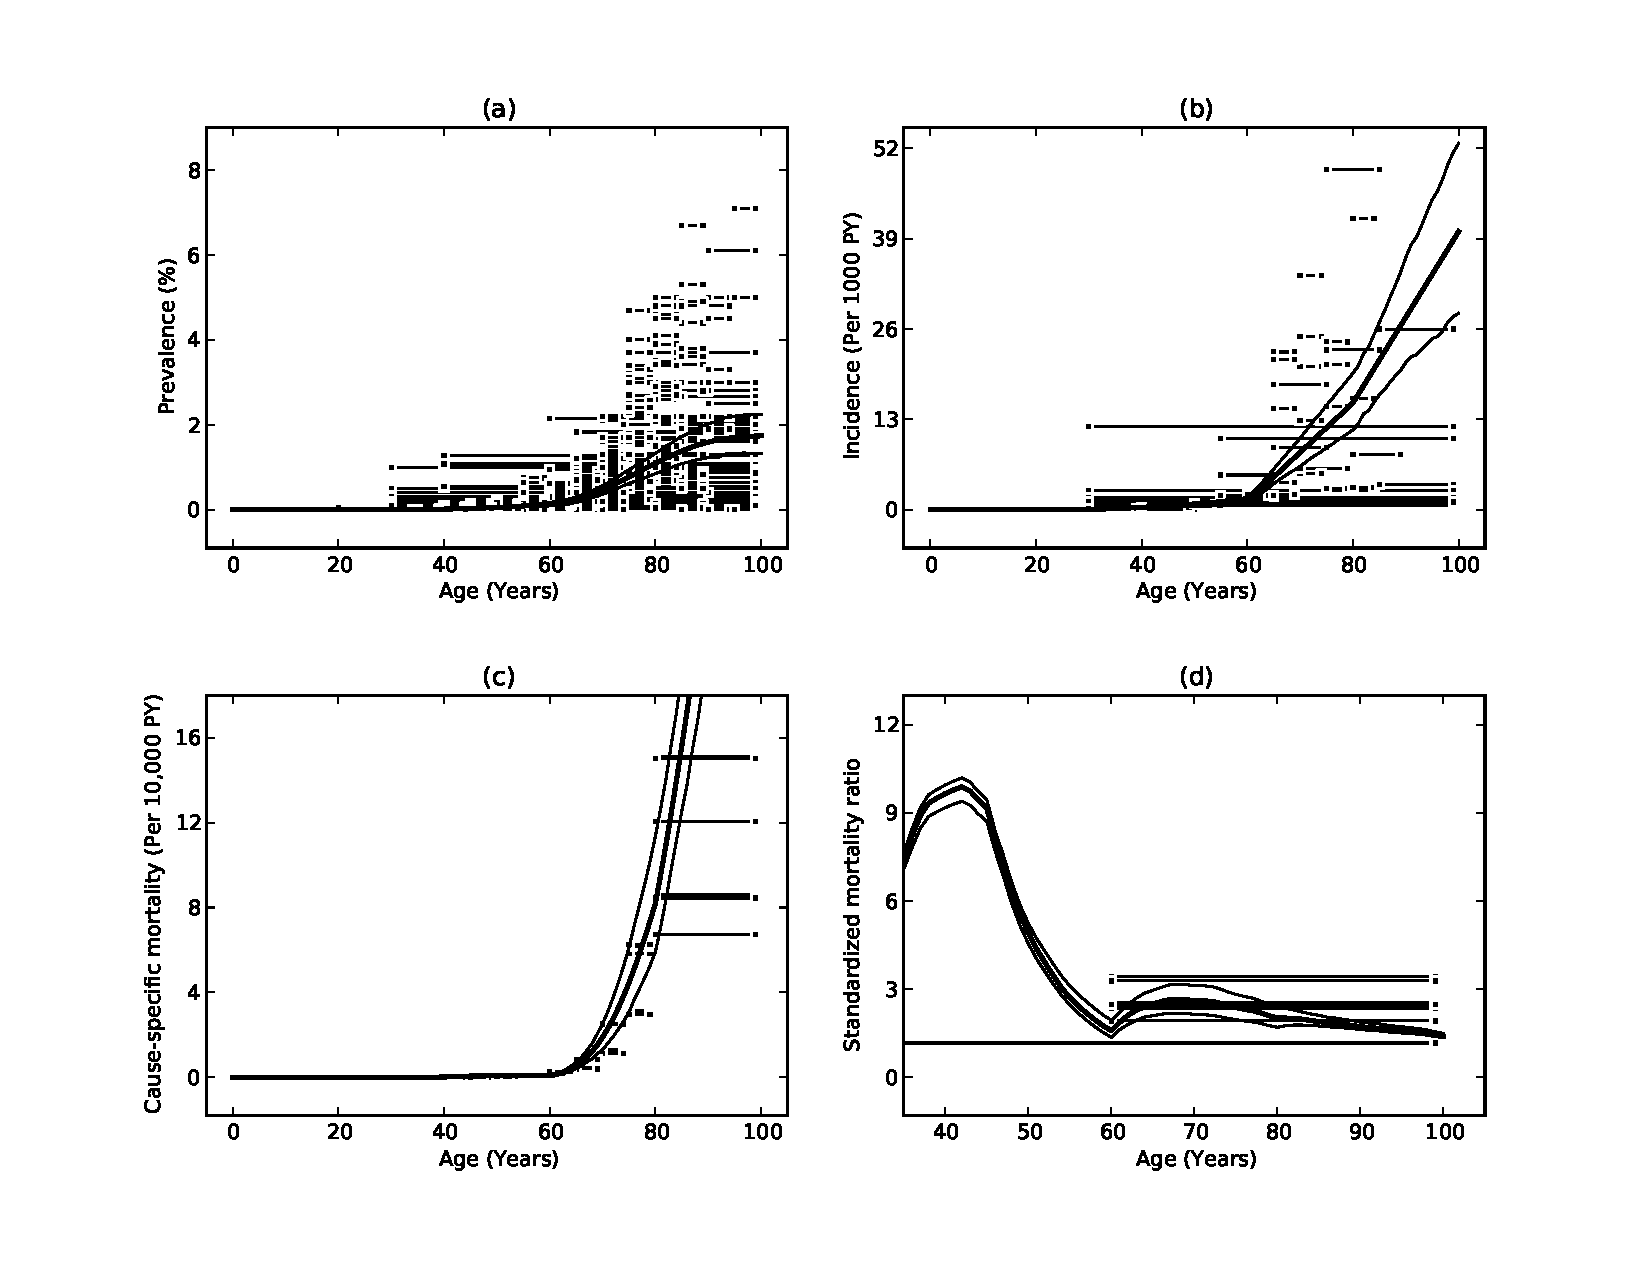
\includegraphics[width=\textwidth]{parkinsons-best.pdf}
            \caption{Estimates of prevalence (panel (a)), incidence (panel (b)), cause-specific mortality (panel (c)) and the standardized mortality ratio of Parkinson's disease in Western European females in 2005.}
            \label{fig:app-parkinsons fit}
        \end{center}
    \end{figure} 